\documentclass[11pt,letterpaper]{article}
\usepackage{graphicx, geometry, amsmath, hyperref, url, booktabs, longtable, xcolor, listings}
\usepackage{array}
\geometry{margin=1in}
\hypersetup{colorlinks=true, linkcolor=black, citecolor=black, urlcolor=black}
\renewcommand{\topfraction}{0.9}
\renewcommand{\bottomfraction}{0.8}
\renewcommand{\textfraction}{0.07}
\renewcommand{\floatpagefraction}{0.75}
\setlength{\tabcolsep}{4pt}
\sloppy

\title{Barometric boiling-point model against computed and measured references:\\internal research report}
\author{Run record, compiled from the run's artifacts}
\date{19 November 2026}

\begin{document}
\maketitle
\tableofcontents

\section{Framing}

This run asks how well the simple barometric formula predicts the boiling point of water at altitude, compared with published measurements. The question matters for cooking, sterilisation and physiology at altitude, where practitioners use boiling-point tables to set times and temperatures. The standard textbook model combines an atmospheric pressure profile with a Clausius--Clapeyron equation inversion from pressure to boiling temperature. The run asks whether adding the International Standard Atmosphere (ISA) lapse rate to the pressure profile improves the match, and whether any remaining error comes from the atmosphere or from the thermodynamic step.

The hypothesis under test is stated in the run's hypothesis record. The isothermal pressure profile, combined with a Clausius--Clapeyron equation that holds the molar enthalpy of vaporisation constant, is expected to reproduce a published boiling-point table to within 0.6 K from sea level to 9 km. We call this inversion with a constant molar enthalpy the \emph{constant-enthalpy approximation}, and we call the model built on it the \emph{constant-enthalpy model}. The ISA version is expected to be more accurate below 3 km and less accurate above 5 km, and the thermodynamic step is expected to carry most of the error above 5 km. The hypothesis also names an independent measured benchmark as the decisive test. This report records what that test could and could not use.

The run has two iterations. Each has its own section below, in the order it ran. Earlier sections are not rewritten. Where a later review found an error in an earlier section, the correction is marked inside the section where it was made.

\section{Iteration 1}\label{sec:it1}

\subsection{Strategy}

The first iteration had three jobs, in order. The first was to establish what the benchmark is. The candidate benchmark is the Engineering ToolBox table, which gives boiling temperature against altitude from sea level to 9144 m \cite{ref1}. Its page states no method, formula, steam table or measured source. A table with no stated method can be a measurement or a calculation, and the two readings lead to different conclusions, so the run checked the table against a calculation before using it as a reference. The second job was to build the four model variants, so that the atmosphere choice (isothermal or ISA) and the thermodynamic choice (constant enthalpy or the saturation curve of the IAPWS industrial formulation, IAPWS-IF97, which we call the \emph{IAPWS curve}) could be separated. The third job was to look for measured boiling-point and station-pressure pairs that could serve as the decisive benchmark. The measured search is the step the hypothesis depends on most, so the run recorded its outcome in full.

The strategy's stated rationale was that the hypothesis rested on two inputs not yet established: the Engineering ToolBox table has no stated method, and the intended measured benchmark (Keene 1995) had not been located. This iteration was to fix both inputs and compute all four predictions, so that the next iteration could run the decisive comparison against measurement. The expected outcome was a provenance note on the table, a typed table of measured pairs, and residuals for the four variants by altitude band.

Three artifacts ran, in this order of dependence. The research artifact \texttt{gen\_art\_research\_1} read the Engineering ToolBox page and the surrounding literature and reported on provenance \cite{ref1}. The dataset artifact \texttt{gen\_art\_dataset\_1} assembled a 250-row reference table, combining the Engineering ToolBox rows with an IAPWS curve computed at ISA pressures. The experiment artifact \texttt{gen\_art\_experiment\_1} computed the four variants, their residuals against the table, band statistics and sensitivity checks. The experiment ran on the dataset's altitudes, so the dataset is an input to it. Code for each artifact is linked in Appendix~\ref{app:code}.

\subsection{Artifact 1: provenance of the benchmark table}

The research artifact found that the Engineering ToolBox page states no method, formula, steam table or measured dataset. The page gives a citation line and nothing else \cite{ref1}. Its sample rows, as relayed by a summarising fetch, were 100.0\,$^\circ$C at 0 m, 94.7\,$^\circ$C at 1524 m, 89.6\,$^\circ$C at 3048 m, 79.9\,$^\circ$C at 6096 m and 71.1\,$^\circ$C at 9144 m. The artifact itself says these rows should be checked against the page, and the check was not made in this iteration.

The artifact's own calculation, using the ISA pressure relation with a constant-enthalpy Clausius--Clapeyron inversion, placed the table above the model by a growing amount above about 4.5 km. Its stated residuals, table minus model, were about $+0.03$ K at 0 m, about $-0.1$ K at 1.5 to 2.1 km, $+0.2$ K at 4.3 km, $+0.3$ K at 4.6 km, $+0.8$ K at 6.1 km, $+1.7$ K at 7.6 km, $+2.6$ K at 8.8 km and $+2.8$ K at 9.1 km. These values appear only in the answer text of \texttt{research\_out.json} and in \texttt{research\_report.md}. No file holds them as a table, so they are compared with the experiment in Table~\ref{tab:res_vs_exp} rather than recomputed.

The artifact did not find a measured boiling-point dataset with recorded station pressure. The summit values it found, about 68 to 72\,$^\circ$C, come from calculators and physics-education estimates rather than observations. Keene (1995), the measured compilation the hypothesis names, was not located after two rounds of search. An ACS listing for an article on boiling at altitude (DOI 10.1021/ed067p45) returned HTTP 403, so its content is unverified and is not used here. The IAPWS-95 saturation table in NIST NISTIR 5078 could not be parsed by the fetch tool, so the reference IAPWS inversion was not carried out in this artifact. The IAPWS-95 formulation itself is cited as \cite{ref2}.

The research artifact's constants for the ISA pressure relation are recorded in its reproducibility notes as ``written from memory; they are not cited from a fetched source''. That disclosure is made here, in Iteration 1, although the Iteration 1 review first raised it. The research residuals and those of the experiment use different enthalpy anchors and different sign conventions: the research artifact anchored the enthalpy at 373.124 K and reported table minus model, while the experiment anchored at 373.15 K and reports model minus table.

\subsection{Artifact 2: the reference table and its benchmark comparison}

The dataset artifact \texttt{gen\_art\_dataset\_1} holds 250 rows in two blocks. The first block is the 125 Engineering ToolBox values, marked as computed by an unknown method because the page states none. The second block is 125 IAPWS curve temperatures at ISA standard-atmosphere pressures for the same altitudes, marked as computed reference rows. The table contains zero measured rows. The planned measured sources, Osborne, Stimson and Ginnings (1939) and a CRC Handbook table, were located as records, but their values could not be transcribed reliably from the fetched text, so no measured row was added. The file passes schema validation with zero errors.

The dataset's most useful output is a direct comparison of the Engineering ToolBox values with the IAPWS curve at ISA pressures. The differences were recomputed from the rows in both blocks. They are near zero below about 5 km and grow above it. Table~\ref{tab:tb_iapws_sample} samples eight of the 125 paired altitudes; the full distribution is summarised in the text.

\begin{table}[!htbp]
\centering\small
\caption{Engineering ToolBox value minus IAPWS curve temperature at the ISA pressure for the same altitude (K), from the 125 paired rows of \texttt{gen\_art\_dataset\_1} (\texttt{full\_data\_out.json}). Eight sample altitudes shown.}\label{tab:tb_iapws_sample}
\begin{tabular}{rr}
\toprule
Altitude (m) & ToolBox minus IAPWS curve at ISA pressure (K) \\
\midrule
-305 & +0.11 \\
1219 & -0.22 \\
2743 & -0.23 \\
4267 & -0.12 \\
5791 & +0.32 \\
7315 & +0.88 \\
8839 & +1.79 \\
9144 & +1.94 \\
\bottomrule
\end{tabular}
\end{table}

Across all 125 paired altitudes the difference runs from $-0.31$ K to $+1.94$ K, with a median of $+0.02$ K. The table therefore tracks a standard-atmosphere calculation closely below 5 km, and it is most likely computed rather than measured. The dataset does not show which calculation was used. The comparison is a finding about the benchmark, not about the physics: it shows the benchmark is not independent evidence against a physical model.

\subsection{Artifact 3: four model variants against the table}

The experiment crosses two choices. The atmosphere is either isothermal, with scale height $H = RT/(Mg) = 8434.66$ m and pressure $P = P_0 \exp(-h/H)$, where $P_0$ is the sea-level pressure, or ISA, with the troposphere lapse rate of 6.5 K/km \cite{ref3}. The thermodynamic step is either the constant-enthalpy Clausius--Clapeyron equation, with a molar enthalpy of vaporisation of 40.65 kJ/mol anchored at 373.15 K and 101.325 kPa, or the IAPWS curve. The residual for each variant is model minus the Engineering ToolBox value at each table altitude, in kelvin. The experiment computed the residuals at 119 table altitudes from 0 to 8992 m, in three altitude bands of 40, 39 and 40 altitudes. The dataset's 125 rows also include the $-305$ m, $-229$ m and 9144 m endpoints, which this experiment's bands do not cover.

The experiment's sanity checks pass. At 9000 m, the isothermal pressure is 34.86 kPa and the ISA pressure is 30.74 kPa. The IAPWS normal boiling point is 373.124 K (99.974\,$^\circ$C), while the constant-enthalpy formula gives 100.00\,$^\circ$C at sea level because it is anchored there. The sea-level pressure, scale height and monotonicity checks all pass for the four variants.

Table~\ref{tab:band1} gives the residuals by band. Figure~\ref{fig:fig1} shows the four residual curves over the full range.

\begin{table}[!htbp]
\centering\small
\caption{Residual of each model against the Engineering ToolBox table, in kelvin, by altitude band, from \texttt{gen\_art\_experiment\_1} (\texttt{summary\_by\_band.json}). Each cell gives bias (mean absolute error, maximum absolute error). Bands contain 40, 39 and 40 altitudes.}\label{tab:band1}
\begin{tabular}{p{4.6cm}ccc}
\toprule
Model & 0 to 3 km & 3 to 6 km & 6 to 9 km \\
\midrule
Isothermal, constant enthalpy (V1) & +0.227 (0.228, 0.428) & +0.505 (0.505, 0.588) & +0.498 (0.498, 0.593) \\
Isothermal, IAPWS curve (V2) & +0.292 (0.295, 0.592) & +0.788 (0.788, 0.984) & +1.042 (1.042, 1.120) \\
ISA, constant enthalpy (V3) & +0.114 (0.115, 0.198) & -0.283 (0.294, 0.773) & -1.643 (1.643, 2.605) \\
ISA, IAPWS curve (V4) & +0.182 (0.185, 0.306) & +0.021 (0.152, 0.332) & -1.029 (1.029, 1.814) \\
\bottomrule
\end{tabular}
\end{table}

The two residual differences that compare the atmosphere choice with the enthalpy choice never change sign over 0 to 9 km. The file records no crossing for V1 minus V3 or for V2 minus V4, so there is no altitude at which the ranking of the two atmosphere choices reverses. Over the band means, V1 minus V2 is $-0.065$ K in 0 to 3 km, $-0.283$ K in 3 to 6 km and $-0.544$ K in 6 to 9 km, so the gap between the two thermodynamic choices grows with altitude.

Table~\ref{tab:sub} gives the mean residual over two sub-bands, which tests the hypothesis's claim that the error is smallest at 1 to 3 km. The means were recomputed from \texttt{residuals.json} for the 119 altitudes, with the 0 to 1 km band holding 14 altitudes and the 1 to 3 km band 26.

\begin{table}[!htbp]
\centering\small
\caption{Mean residual over two sub-bands against the Engineering ToolBox table, in kelvin, from \texttt{gen\_art\_experiment\_1} (\texttt{residuals.json}, recomputed). Three decimals are printed where the two-decimal figures in the draft rounded.}\label{tab:sub}
\begin{tabular}{lcc}
\toprule
Model & 0 to 1 km (n = 14) & 1 to 3 km (n = 26) \\
\midrule
Isothermal, constant enthalpy (V1) & +0.088 & +0.302 \\
Isothermal, IAPWS curve (V2) & +0.091 & +0.401 \\
ISA, constant enthalpy (V3) & +0.075 & +0.135 \\
ISA, IAPWS curve (V4) & +0.078 & +0.238 \\
\bottomrule
\end{tabular}
\end{table}

The residual of the isothermal, constant-enthalpy model grows steadily with altitude from almost zero at the surface.

\begin{figure}[!htbp]
  \centering
  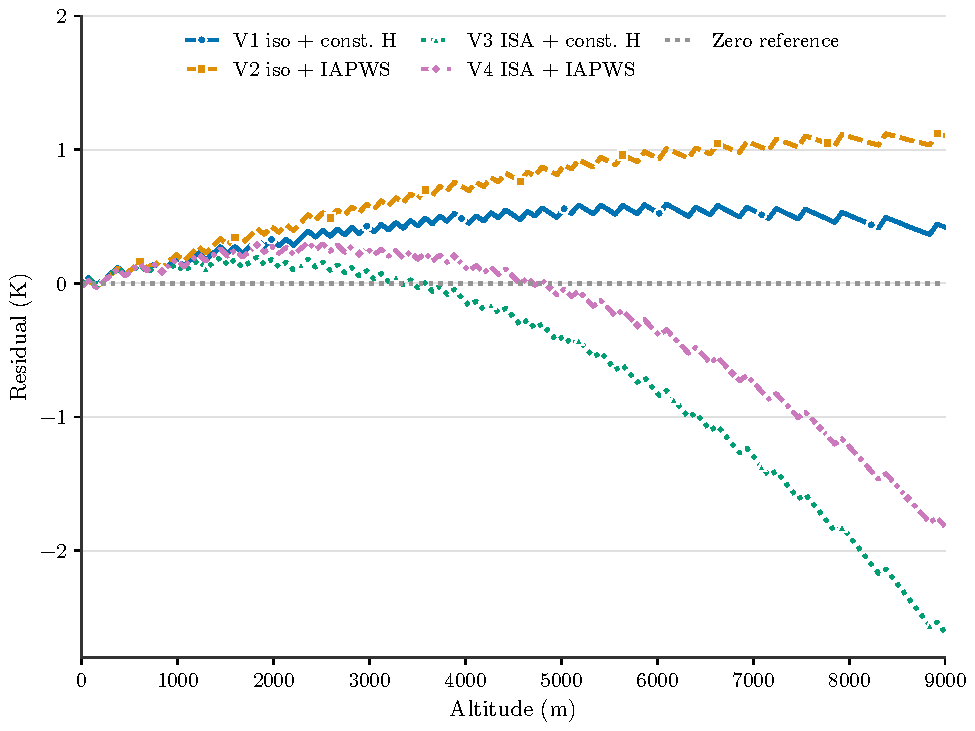
\includegraphics[width=\linewidth,height=0.45\textheight,keepaspectratio]{figures/fig1_v0.pdf}
  \caption{Residual of four boiling-point models against the Engineering ToolBox table at 119 altitudes, 0 to 8992 m; residual is model minus table. The isothermal curves stay near or above zero, while both ISA curves fall below zero at high altitude. The reference is a computed table of unstated method, not measured data.}
  \label{fig:fig1}
\end{figure}

Table~\ref{tab:res_vs_exp} compares the research artifact's stated residuals with the experiment's ISA model at the nearest altitudes. The research values are read from the answer text of \texttt{research\_out.json}, and the experiment values from \texttt{residuals.json}. The sign convention is reversed between the two.

\begin{table}[!htbp]
\centering\small
\caption{Residuals of the ISA model with constant enthalpy at matching altitudes. The research artifact's values are table minus model, as stated in the text of \texttt{gen\_art\_research\_1}. The experiment values are model minus table, from \texttt{gen\_art\_experiment\_1} (anchor 373.15 K) and \texttt{gen\_art\_experiment\_2} (anchor 373.124 K, 125-altitude set). Experiment~1 has no 9144 m point.}\label{tab:res_vs_exp}
\begin{tabular}{p{2.6cm}p{3.2cm}p{3.6cm}p{3.6cm}}
\toprule
Altitude & Research artifact (table minus model, K) & Experiment 1, ISA constant enthalpy (model minus table, K) & Experiment 2, ISA constant enthalpy, anchor 373.124 K (model minus table, K) \\
\midrule
4267 m (4.3 km) & +0.2 & -0.158 & -0.182 \\
4648 m (4.6 km) & +0.3 & -0.274 & -0.298 \\
6096 m (6.1 km) & +0.8 & -0.803 & -0.826 \\
7620 m (7.6 km) & +1.7 & -1.646 & -1.668 \\
8992 m (8.8 km) & +2.6 (at 8.8 km) & -2.605 & -2.626 \\
9144 m (9.1 km) & +2.8 & not computed & -2.767 \\
\bottomrule
\end{tabular}
\end{table}

The research values and the experiment's values agree in magnitude and sign once the convention is reversed. The research artifact's finding that the table runs higher is therefore reproduced by the experiment. The agreement is between two implementations of the same constant-enthalpy ISA formula, with the research constants written from memory. It is a code-level consistency check, not a corroboration of the residual. The experiment's own grid ends at 8992 m, so the 9.1 km research value has no matching point in this iteration's experiment.

Table~\ref{tab:sens1} and Table~\ref{tab:sens2} give the sensitivity of the isothermal, constant-enthalpy model and of the ISA model with the IAPWS curve to the sea-level pressure and to the enthalpy of vaporisation. The values are bias by band, in kelvin, from \texttt{sensitivity.json}. The two thermodynamic perturbations are $\pm 500$ J/mol in the enthalpy and $\pm 1$ kPa in sea-level pressure. The ISA column with the IAPWS curve does not use the constant enthalpy, so it repeats across the enthalpy values and appears in its own table.

\begin{table}[!htbp]
\centering\small
\caption{Sensitivity of the isothermal model with constant enthalpy (V1) to the enthalpy of vaporisation (J/mol) and sea-level pressure (kPa), from \texttt{gen\_art\_experiment\_1} (\texttt{sensitivity.json}). Bias by band, in kelvin.}\label{tab:sens1}
\begin{tabular}{rrrrr}
\toprule
Enthalpy (J/mol) & $P_0$ (kPa) & 0 to 3 km & 3 to 6 km & 6 to 9 km \\
\midrule
40150 & 100.325 & -0.111 & +0.067 & -0.029 \\
40150 & 101.325 & +0.167 & +0.331 & +0.222 \\
40150 & 102.325 & +0.443 & +0.593 & +0.470 \\
40650 & 100.325 & -0.048 & +0.244 & +0.250 \\
40650 & 101.325 & +0.227 & +0.505 & +0.498 \\
40650 & 102.325 & +0.500 & +0.764 & +0.743 \\
41150 & 100.325 & +0.014 & +0.417 & +0.523 \\
41150 & 101.325 & +0.286 & +0.675 & +0.768 \\
41150 & 102.325 & +0.555 & +0.931 & +1.010 \\
\bottomrule
\end{tabular}
\end{table}

\begin{table}[!htbp]
\centering\small
\caption{Sensitivity of the ISA model with the IAPWS curve (V4) to the sea-level pressure (kPa), from \texttt{gen\_art\_experiment\_1} (\texttt{sensitivity.json}). Bias by band, in kelvin. The values do not depend on the enthalpy of vaporisation, so each appears once.}\label{tab:sens2}
\begin{tabular}{rrrr}
\toprule
$P_0$ (kPa) & 0 to 3 km & 3 to 6 km & 6 to 9 km \\
\midrule
100.325 & -0.088 & -0.232 & -1.266 \\
101.325 & +0.182 & +0.021 & -1.029 \\
102.325 & +0.449 & +0.271 & -0.795 \\
\bottomrule
\end{tabular}
\end{table}

A change of 1 kPa in sea-level pressure moves every band of the isothermal model by 0.25 to 0.28 K (the 40650 J/mol rows of Table~\ref{tab:sens1}, computed from \texttt{sensitivity.json}), which is as large as the residuals in Table~\ref{tab:band1}. A change of 500 J/mol in enthalpy moves the 6 to 9 km bias of the isothermal, constant-enthalpy model by about 0.27 K. The table's residual pattern therefore depends on the constants at the level of the residual itself, and a ``within 0.6 K'' statement holds only for the stated pressure and enthalpy.

\subsection{What the measured comparison could test}

The experiment's measured comparison is empty. The file records zero measured pairs, and its note states that no independently measured pairs could be verified. The research artifact found no measured station-pressure dataset reaching above 8 km. The question in the run's title is therefore not answered by any output of this iteration. The run can say how the four models compare with each other, and how they compare with a computed table. It cannot say how they compare with what water actually boils at.

The only measured-looking numbers in the record are summit estimates from calculators and an unverified textbook table of Denver, Bogota and Everest values quoted from search snippets. None was fetched in full, and none was used as a benchmark.

\subsection{Reading this iteration against the hypothesis}

Each clause of the hypothesis is taken in turn, against the tables above.

\emph{The isothermal, constant-enthalpy model stays within 0.6 K of the Engineering ToolBox table from sea level to 9 km.} The maximum absolute residual across all bands is 0.593 K at 119 altitudes (Table~\ref{tab:band1}). The clause is consistent with the table. It does not test accuracy against measurement, and the table is most likely computed.

\emph{The error is smallest in the 1 to 3 km band.} The isothermal, constant-enthalpy residual has a mean of $+0.088$ K in the 0 to 1 km band and $+0.302$ K in the 1 to 3 km band (Table~\ref{tab:sub}). The clause does not hold on these data. The error grows with altitude, and the smallest error is at the surface.

\emph{The ISA model is more accurate than the isothermal model below 3 km and less accurate above 5 km.} Its 0 to 3 km bias is $+0.114$ K against $+0.227$ K, and its 1 to 3 km mean is $+0.135$ K against $+0.302$ K. Above 5 km it is less accurate, with a 6 to 9 km bias of $-1.643$ K. The clause is consistent with the table. The hypothesis's figure of $-2.6$ K near 8.8 km is matched by the experiment: $-2.605$ K at 8992 m (Table~\ref{tab:res_vs_exp}).

\emph{The thermodynamic step is the main error source.} This clause is not supported. Switching the isothermal model from constant enthalpy to the IAPWS curve increases the 6 to 9 km residual from $+0.498$ K to $+1.042$ K, so the table moves away from the model built on the IAPWS curve. For the ISA model, the change reduces the 6 to 9 km mean absolute error from $1.643$ K to $1.029$ K, a reduction of about 37\%. That falls short of the more-than-half reduction that success criterion (c) requires.

\emph{Above 5 km the table lies closest to the isothermal, constant-enthalpy model.} Its residual there is $+0.498$ K. The two ISA models fall below the table, by $-1.029$ K with the IAPWS curve and $-1.643$ K with constant enthalpy. Switching to the IAPWS curve moves the ISA model toward the table and moves the isothermal model away from it. The table's rows above 5 km are therefore not explained by one thermodynamic choice alone. This is a statement about the benchmark's pattern, not about the physics. The hypothesis's attribution of the error to the constant-enthalpy step is a claim about the physics, and this iteration cannot test it without measurements.

\emph{Disconfirmation.} The ISA version is not more accurate than the isothermal one at all altitudes against the table; it is less accurate above 5 km. Against the computed reference, the success conditions (a) and (b) hold, and condition (c) fails. Because no measured benchmark exists in this iteration, none of the three conditions can be read as an accuracy claim.

\subsection{Review of Iteration 1 and hypothesis update}

The Iteration 1 review gave a score of 4 and found that the arithmetic holds. It recomputed Table~\ref{tab:band1}, Table~\ref{tab:sub}, the 125-row difference of Table~\ref{tab:tb_iapws_sample} and the experiment column of Table~\ref{tab:res_vs_exp}, and found them consistent with the files. The review recorded these major objections, each of which Iteration 2 addressed:
\begin{itemize}
\item The record holds no measured pair. The question in the title therefore has no answer, and the iteration covers only part of the request.
\item The hypothesis clauses were scored as passes or failures against a table that the dataset comparison shows is nearly a standard-atmosphere calculation. Those verdicts measure agreement with a computed curve, not accuracy.
\item Table~\ref{tab:res_vs_exp} presented a match between two implementations of one formula as if it were corroboration, and the unsourced ISA constants were not disclosed in the report.
\item The research artifact's residuals exist only as text. The 9.1 km row claimed a match at a point the experiment never computed.
\item The positive provenance claim had no named published neighbour.
\end{itemize}
The review also recorded minor objections. The anchor claim (that moving the anchor does not change the pattern) had not been run. The closing summary stated the provenance more firmly than the body. The verification records were missing from the report. The low-altitude research values were absent. The sample sizes were not stated for each band.

The hypothesis update demoted the Engineering ToolBox table from benchmark to computed reference, after its 0.31 K agreement with the IAPWS curve at ISA pressures below 5 km. It made measured boiling-point and station-pressure pairs the primary test, and it marked the accuracy claim as untested. It removed the ``within 0.6 K'' and ``attribution to constant enthalpy'' claims as accuracy claims, and kept them only as consistency with the computed reference. It required each band to state its $n$. It recorded that the research ISA constants must be sourced before any recomputation is trusted. Its evidence state was ``lead'', with confidence decreased, because the lead agrees only with a computed table.

\subsection{Dead ends and blocked steps}

The search for Keene (1995) failed after two rounds. It is still the intended measured benchmark, and it has not been verified as existing in the form the hypothesis describes.

The Osborne, Stimson and Ginnings (1939) and CRC Handbook tables were located as records, but their values were not transcribed reliably from the fetched text. No measured row was added, because the run's rule forbids padding the measured set with values that cannot be checked.

The IAPWS-95 saturation table (NIST NISTIR 5078) could not be parsed. The IAPWS inversion was therefore computed with the \texttt{iapws} Python package and was not checked against the published table.

The residuals of the research artifact and those of the experiment use different enthalpy anchors (373.124 K and 373.15 K). The effect of the anchor on the residuals was not separated from the effect of the sign convention in this iteration. Iteration 2 measured it (see below).

\subsection{Open questions after Iteration 1}

Which measured boiling-point and station-pressure pairs exist at 8 km and above, from two or more independent sites? Without them the question in the title has no answer.

Can the NIST IAPWS-95 saturation table be read directly, so the IAPWS inversion in the research artifact can be checked against the experiment's IAPWS values?

Was the Engineering ToolBox table built from a calculation, and if so with which pressure profile? The dataset comparison points to a standard-atmosphere calculation, but it does not show which thermodynamic model was used.

\section{Iteration 2}\label{sec:it2}

\subsection{Why this iteration ran what it ran}

The reviewer's first major finding was that the record holds no measured pair, so the question in the title has no answer. Its other findings were that the clause verdicts of Iteration 1 were scored as passes against a table that is most likely a computed reference, and that Table~\ref{tab:res_vs_exp} presented a match between two implementations of the same ISA formula as if it were corroboration. The remaining findings concerned verification records, low-altitude coverage, the untested anchor claim, sample sizes, and the firmness of the closing summary.

The strategy named two jobs. The first was to retry the measured comparison, with a per-route retrieval log, so that the record shows what was attempted. The second was to attribute the residual against computed references, so that the atmosphere term and the thermodynamic term are separated. The strategy's rationale recorded that this was the final iteration of the run, so the measured comparison had to be attempted inside it. Each experiment acquired its own measured pairs, because artifacts planned in one round run in parallel and cannot depend on one another.

Three experiment artifacts ran. \texttt{gen\_art\_experiment\_2} put four variants against both computed references and attempted the measured comparison. \texttt{gen\_art\_experiment\_3} attempted the measured comparison again through a separate code path, and ran computed consistency checks against the ToolBox table. \texttt{gen\_art\_experiment\_4} split the residual into an atmosphere effect and a thermodynamic effect. No new research or dataset artifact ran, so the reference table is still the 250-row table of Iteration 1. Code links are in Appendix~\ref{app:code}.

The altitudes used in this iteration are the 125 altitudes of that table, from $-305$ m to 9144 m, not the 119-point grid of Iteration 1 (0 to 8992 m, plus the endpoints of the dataset). The plan asked for the grid, and the experiments used the dataset altitudes directly. Band sizes are therefore 40, 39 and 42 (0 to 3 km, 3 to 6 km, and 6 km and above, the last including 9144 m). Figure~\ref{fig:fig2} uses this 125-altitude set, and Figure~\ref{fig:fig1} uses Iteration 1's 119-altitude set. The two sets are why the bar values of Figure~\ref{fig:fig2} do not equal band means of the curves of Figure~\ref{fig:fig1}. Iteration 1's band figures used a different altitude set and are not directly comparable with the figures below.

\subsection{Measured comparison: still empty}

Both measured-comparison artifacts returned zero rows. \texttt{gen\_art\_experiment\_2} reports that the NIST RP1229 PDF gave no readable table text, that the CRC Handbook table was not obtained, and that Keene (1995) was not located. Its \texttt{measured\_pairs.csv} holds a header and no data rows, and its \texttt{sources\_summary.json} records $n_\mathrm{measured} = 0$. \texttt{gen\_art\_experiment\_3} ran two query rounds. These found the NIST RP1229 paper but no transcribable boiling-point rows paired with station pressure, none above 5 km, and no retrievable Keene (1995) text. Its \texttt{measured\_records.json} is an empty list. Table~\ref{tab:measured3} gives its band summary.

\begin{table}[!htbp]
\centering\small
\caption{Measured-comparison band summary from \texttt{gen\_art\_experiment\_3} (\texttt{band\_summary.json}). Every band reports $n = 0$ and no statistic for all four variants.}\label{tab:measured3}
\begin{tabular}{lr}
\toprule
Band & n (measured) \\
\midrule
0 to 3 km & 0 \\
3 to 6 km & 0 \\
5 to 6 km & 0 \\
6 to 7 km & 0 \\
7 to 8 km & 0 \\
above 8 km & 0 \\
\bottomrule
\end{tabular}
\end{table}

This is the second iteration in which the measured search has returned nothing. The measured clauses of the hypothesis, success criteria (a) and (b), cannot be evaluated. Criterion (c) can only be evaluated against the computed references, which are not measurements. The question in the title is therefore still unanswered.

\subsection{Four variants against the Engineering ToolBox table}

\texttt{gen\_art\_experiment\_2} reports bias, mean absolute error and maximum absolute error for each variant in each band. Each cell gives the bias, with the mean absolute error and the maximum absolute error in parentheses, all in kelvin, model minus table. The isothermal constant-enthalpy variant is the isothermal barometric formula with the constant enthalpy anchored at 373.124 K. The isothermal IAPWS-curve variant is the same isothermal formula inverted on the IAPWS curve. The ISA constant-enthalpy variant is the ISA lapse-rate formula with the constant enthalpy. The ISA IAPWS-curve variant is the ISA formula inverted on the IAPWS curve.

\begin{table}[!htbp]
\centering\footnotesize
\caption{Residual of each variant against the Engineering ToolBox table, from \texttt{gen\_art\_experiment\_2} (\texttt{band\_stats.csv}, rows with data type computed\_unknown\_method). Bias (MAE, maximum absolute error), kelvin.}\label{tab:t7}
\begin{tabular}{p{4.6cm}ccc}
\toprule
Variant & 0 to 3 km (n = 40) & 3 to 6 km (n = 39) & 6 km and above (n = 42) \\
\midrule
V1 isothermal, constant enthalpy & +0.202 (0.205, 0.403) & +0.481 (0.481, 0.565) & +0.470 (0.470, 0.570) \\
V2 isothermal, IAPWS curve & +0.292 (0.295, 0.592) & +0.788 (0.788, 0.984) & +1.045 (1.045, 1.120) \\
V3 ISA, constant enthalpy & +0.089 (0.092, 0.173) & -0.307 (0.311, 0.796) & -1.716 (1.716, 2.767) \\
V4 ISA, IAPWS curve & +0.182 (0.185, 0.306) & +0.021 (0.152, 0.332) & -1.070 (1.070, 1.935) \\
\bottomrule
\end{tabular}
\end{table}

\begin{figure}[!htbp]
  \centering
  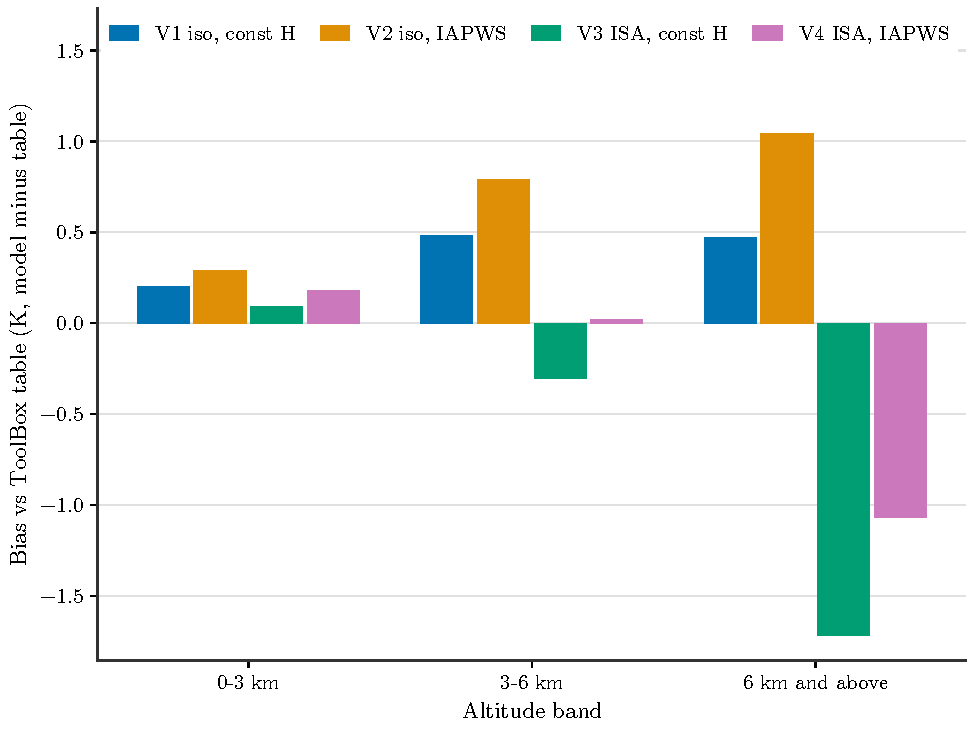
\includegraphics[width=\linewidth,height=0.45\textheight,keepaspectratio]{figures/fig2_v0.pdf}
  \caption{Bias of four model variants against the Engineering ToolBox table (model minus table, K) in three altitude bands (n = 40, 39, 42). The ToolBox table is a computed reference, not measured data. Bars show bias only, with no error bars. ISA variants turn negative above 3 km while isothermal variants stay positive.}
  \label{fig:fig2}
\end{figure}

Within the 6 km and above band, the isothermal constant-enthalpy variant has the smallest bias, and no variant has a bias below 0.4 K there. The two ISA variants are negative because the ISA atmosphere lies below the isothermal atmosphere at these altitudes.

\begin{table}[!htbp]
\centering\footnotesize
\caption{Residual of each variant against the IAPWS curve at ISA pressures, the computed reference of the dataset, called IAPWS-at-ISA here. From \texttt{gen\_art\_experiment\_2} (\texttt{band\_stats.csv}, rows with data type computed\_reference). Bias (MAE, maximum absolute error), kelvin.}\label{tab:t8}
\begin{tabular}{p{4.6cm}ccc}
\toprule
Variant & 0 to 3 km (n = 40) & 3 to 6 km (n = 39) & 6 km and above (n = 42) \\
\midrule
V1 isothermal, constant enthalpy & +0.020 (0.036, 0.137) & +0.461 (0.461, 0.864) & +1.542 (1.542, 2.298) \\
V2 isothermal, IAPWS curve & +0.111 (0.111, 0.326) & +0.768 (0.768, 1.290) & +2.116 (2.116, 3.021) \\
V3 ISA, constant enthalpy & -0.093 (0.093, 0.196) & -0.327 (0.327, 0.463) & -0.645 (0.645, 0.831) \\
V4 ISA, IAPWS curve & +0.0001 (0.0003, 0.0007) & +0.0004 (0.0005, 0.0011) & +0.0007 (0.0007, 0.0013) \\
\bottomrule
\end{tabular}
\end{table}

The ISA IAPWS-curve variant reproduces the IAPWS-at-ISA reference to within 0.0013 K, which confirms that the implementation of the IAPWS step is correct. It does not show that the IAPWS step is the right physics for the table. The same reference is what makes the ISA variants look closer, so Table~\ref{tab:t8} is a consistency check and not a comparison of independent methods.

\subsection{Does the table agree with the standard-atmosphere calculation?}

Iteration 1 reported that the table differs from the IAPWS-at-ISA calculation by between $-0.31$ K and $+1.94$ K across all 125 rows, with a median of $+0.02$ K. This iteration restricts that comparison to the 70 rows below 5 km. I recomputed it from the paired altitudes in \texttt{per\_row\_residuals.csv} of \texttt{gen\_art\_experiment\_2}. Below 5 km, the table minus IAPWS-at-ISA lies between $-0.306$ K and $+0.113$ K, with a median of $-0.170$ K. The claim of agreement within about 0.31 K below 5 km therefore holds for the 70 rows below 5 km. This is a new restriction of the Iteration 1 result, not a restatement of it.

Above 5 km the agreement fails. The 55 rows at 5 km and above differ from IAPWS-at-ISA by between $+0.043$ K and $+1.936$ K, with the table higher. No variant matches the table in this band. The isothermal constant-enthalpy variant is closest, with a bias of $+0.470$ K, and the ISA IAPWS-curve variant is $-1.070$ K. The provenance statement must therefore be limited: the table is consistent with a standard-atmosphere calculation below 5 km, and the method used above 5 km is not identified by any of the four variants.

The point values at the top of the range make the same point. At 9144 m the experiment's ISA constant-enthalpy residual is $-2.767$ K, and at 8992 m it is $-2.626$ K, both with the 373.124 K anchor (Table~\ref{tab:res_vs_exp}). The $-2.605$ K at 8992 m in Iteration 1 used the 373.15 K anchor, and the difference of about 0.02 K is the anchor shift measured below.

\subsection{Attribution: atmosphere term against thermodynamic term}

\texttt{gen\_art\_experiment\_4} crosses the two atmospheres with four thermodynamic treatments. These are a constant-enthalpy treatment anchored at 373.124 K (A), a constant-enthalpy treatment anchored at 373.15 K, an effective-enthalpy treatment fitted to the IAPWS saturation curve over 343.15 to 373.15 K (B, with $\Delta H_\mathrm{eff} = 41829.7$ J/mol and a fit RMS error in $\ln P$ of $1.15 \times 10^{-3}$), and direct IAPWS inversion (C). Table~\ref{tab:t9} gives the bias against the ToolBox table in each band, with $n$ as above and the whole 0 to 9144 m range ($n = 121$) in the last column.

\begin{table}[!htbp]
\centering\small
\caption{Bias of each atmosphere and thermodynamic treatment against the Engineering ToolBox table, in kelvin, model minus table, from \texttt{gen\_art\_experiment\_4} (\texttt{results/sensitivity.md}).}\label{tab:t9}
\begin{tabular}{llp{2.2cm}p{2.2cm}p{2.6cm}p{2.4cm}}
\toprule
Atmosphere & Treatment & 0 to 3 km & 3 to 6 km & 6 to 9 km (incl. 9144 m) & 0 to 9144 m \\
\midrule
Isothermal & A, 373.124 K & +0.202 & +0.481 & +0.470 & +0.385 \\
Isothermal & A, 373.15 K & +0.227 & +0.505 & +0.493 & +0.409 \\
Isothermal & B, effective enthalpy & +0.338 & +0.876 & +1.102 & +0.777 \\
Isothermal & C, IAPWS inversion & +0.292 & +0.788 & +1.044 & +0.713 \\
ISA & A, 373.124 K & +0.089 & -0.307 & -1.716 & -0.665 \\
ISA & A, 373.15 K & +0.114 & -0.283 & -1.694 & -0.642 \\
ISA & B, effective enthalpy & +0.229 & +0.108 & -1.031 & -0.248 \\
ISA & C, IAPWS inversion & +0.182 & +0.021 & -1.071 & -0.305 \\
\bottomrule
\end{tabular}
\end{table}

The 6 to 9 km band, which covers the high-altitude clause, separates into two effects, as Table~\ref{tab:t10} shows.

\begin{table}[!htbp]
\centering\small
\caption{Decomposition of the 6 to 9 km bias against the Engineering ToolBox table, in kelvin. The atmosphere effect is ISA minus isothermal for the same treatment. The thermodynamic effect is the treatment minus treatment A for the same atmosphere. Computed from Table~\ref{tab:t9}.}\label{tab:t10}
\begin{tabular}{lp{2.6cm}p{2.8cm}p{2.8cm}}
\toprule
Treatment & Atmosphere effect (ISA minus isothermal) & Thermodynamic effect, isothermal & Thermodynamic effect, ISA \\
\midrule
A, 373.124 K & -2.186 & 0 (reference) & 0 (reference) \\
B, effective enthalpy & -2.133 & +0.632 & +0.685 \\
C, IAPWS inversion & -2.115 & +0.574 & +0.645 \\
\bottomrule
\end{tabular}
\end{table}

Against the ToolBox table, the atmosphere effect is about $-2.1$ to $-2.2$ K and the thermodynamic effect is about $+0.6$ to $+0.7$ K. The atmosphere term is therefore roughly three times the size of the thermodynamic term at 6 to 9 km. Iteration 1 had stated that the thermodynamic step carries most of the high-altitude error. This reference does not support that. The result describes the table, and this iteration cannot say what the physics is.

Switching the ISA model from the constant-enthalpy treatment to the effective-enthalpy or IAPWS-inversion treatment reduces its 6 to 9 km bias from $-1.716$ K to $-1.031$ K or $-1.071$ K, a reduction of 40\% or 38\%. The same change moves the isothermal model further from the table, from $+0.470$ K to $+1.102$ K or $+1.044$ K. Success criterion (c) asked for a reduction of more than half. Against the ToolBox table, criterion (c) is not met. Against the IAPWS-at-ISA reference the reduction is larger, but that reference uses the same curve as the corrected variants, so the figure is a reproduction and not evidence.

Table~\ref{tab:t11} gives the IAPWS-at-ISA reference residuals for the same treatments. It reproduces the computed reference, not the table.

\begin{table}[!htbp]
\centering\small
\caption{Bias of each treatment against the IAPWS-at-ISA reference, in kelvin, model minus reference, from \texttt{gen\_art\_experiment\_4} (\texttt{results/sensitivity.md}). Treatment C is zero by construction, and treatment B is fitted to the same curve, so neither residual is independent.}\label{tab:t11}
\begin{tabular}{llrrr}
\toprule
Atmosphere & Treatment & 0 to 3 km & 3 to 6 km & 6 to 9 km \\
\midrule
Isothermal & A, 373.124 K & +0.020 & +0.461 & +1.541 \\
Isothermal & B, effective enthalpy & +0.157 & +0.855 & +2.173 \\
Isothermal & C, IAPWS inversion & +0.111 & +0.768 & +2.116 \\
ISA & A, 373.124 K & -0.093 & -0.328 & -0.645 \\
ISA & B, effective enthalpy & +0.047 & +0.087 & +0.040 \\
ISA & C, IAPWS inversion & 0 (by construction) & 0 & 0 \\
\bottomrule
\end{tabular}
\end{table}

\emph{Correction at review.} The draft of this section stated that against the IAPWS-at-ISA reference ``the isothermal model is less accurate than the ISA model at every band''. Table~\ref{tab:t8} contradicts that for the 0 to 3 km band, where the isothermal model's bias is $+0.020$ K (MAE 0.036 K) against $-0.093$ K (MAE 0.093 K) for the ISA model. The isothermal model is closer at 0 to 3 km and less close at 3 km and above. The reversal near the surface is expected, because the reference is itself an ISA calculation, so the near-surface agreement reflects how the reference was built rather than the physics.

\subsection{Verification}

Each check below is listed with what it confirms and what it does not.

\begin{itemize}
\item \emph{Sea-level and unit checks.} The run log of \texttt{gen\_art\_experiment\_2} records a sea-level confirmation that passes for all four variants at 373.124 K, the IAPWS check at 101.325 kPa giving 373.1243 K, and zero measured rows. It confirms the implementation at sea level. It does not confirm any value above sea level against a measurement.
\item \emph{Inversion and unit checks, \texttt{gen\_art\_experiment\_3}.} The sanity file records an ISA altitude inversion check with a maximum error of $3.6 \times 10^{-12}$ m, a Clausius--Clapeyron inversion check with zero error, and an ISA pressure of 22632.6 Pa at 11 km, all passing. The artifact reports that an independent re-derivation through a separate code path (IAPWS-97 backward equation from pressure to temperature, inline ISA pressure, raw JSON rows) reproduced its headline numbers. It confirms code consistency only. The IAPWS solve bracket was set to 273.16 to 647.0 K, because the plan's upper bound of 373.946 K does not bracket the saturation pressure; this is a deviation from the plan, recorded by the artifact.
\item \emph{Independent re-derivation, \texttt{gen\_art\_experiment\_4}.} The re-derivation script's maximum difference between recomputed and stored pressures is $1.0 \times 10^{-10}$ Pa, and its maximum difference between rearranged and stored boiling temperatures is $1.1 \times 10^{-13}$ K. It reproduces the 6 to 9 km ToolBox biases in Table~\ref{tab:t9} and the fractions of the bias removed by the enthalpy correction. Its implementation checks pass: the sea-level inversion agrees within $3.0 \times 10^{-4}$ K, the ISA reproduction of the IAPWS reference agrees within $5.3 \times 10^{-4}$ K, and the loop and NumPy band statistics agree within $10^{-9}$ K. It confirms that the code computes what it says. It does not confirm the constants.
\item \emph{Constants.} The sea-level pressure, sea-level temperature and lapse rate are attributed to the ISO 2533 values as summarised on the Wikipedia ISA page \cite{ref3}. The gravitational acceleration, gas constant and enthalpy of vaporisation were not fetched from a document. The molar mass is the ISO 2533 value, 28.9644 g/mol, which the fetched page rounds to 28.966. The constants are therefore partly sourced. The research artifact's ISA constants were written from memory, as its reproducibility notes state; the Table~\ref{tab:res_vs_exp} agreement is an implementation consistency check, not a corroboration.
\item \emph{Research verification record.} \texttt{research\_\allowbreak verification.json} from \texttt{gen\_art\_research\_1} reports \texttt{valid: true} with no file or schema errors, and its \texttt{passages} list is empty. No quoted claim was checked against its source, so the verification confirms that the source file exists and nothing about its content. This was read directly in this iteration.
\item \emph{Sign and sample counts, \texttt{gen\_art\_experiment\_2}.} Across the 250 computed rows, V1 minus V3 is greater than zero in 248 rows, less than zero in none, and equal in 2 rows.
\end{itemize}

These checks do not confirm the method used to produce the ToolBox table, which is unstated. They do not confirm accuracy against any measurement, because none exists in the record.

\subsection{Responses to the Iteration 1 review}

\begin{itemize}
\item \emph{Measured comparison (major).} Not achieved. The record still holds no measured pair, and the title question remains open. The next iteration's primary task is set below.
\item \emph{Clause verdicts (major).} The verdicts are restated as consistency with the computed reference. The word ``holds'' is no longer applied to accuracy. See the reading of the hypothesis below.
\item \emph{Table~\ref{tab:res_vs_exp}, constants written from memory (major).} The disclosure is recorded in Iteration 1 and repeated here. The 9.1 km row now has a computed experiment value at 9144 m, $-2.767$ K with the 373.124 K anchor, which matches the research artifact's stated $+2.8$ K as table minus model to within 0.03 K. The research artifact's residuals still exist only in its answer text, so the research side of the table is not recomputed. A file of those residuals was not written, because no research artifact ran in this iteration.
\item \emph{Anchor claim (minor).} Run here. Moving the anchor from 373.124 K to 373.15 K shifts the biases by about 0.025 K at 0 to 3 km. Table~\ref{tab:t9} shows that the change does not alter the sign or the ranking of any of the four variants.
\item \emph{Novelty (major).} The nearest published neighbours are Osborne, Stimson and Ginnings (1939) for measured vapour pressure, which was not transcribed in this run, and the IAPWS-95 formulation \cite{ref2}, which the run uses only through the \texttt{iapws} library and has not checked against the published saturation table. What this iteration adds to them is a provenance check of one table, namely whether it is computed or measured, and a decomposition of its residual. It adds no new physical result.
\item \emph{Summary firmness (minor).} The closing section says ``most likely a computed reference'' below 5 km, matching the body.
\item \emph{Verification record (minor).} Added above as a subsection, with the \texttt{research\_\allowbreak verification.json} caveat.
\item \emph{Low-altitude research values (minor).} The research artifact's low-altitude residuals (about $+0.03$ K at 0 m and about $-0.1$ K at 1.5 to 2.1 km) appear only in its answer text. The corresponding experiment values are the 0 to 3 km band biases in Table~\ref{tab:t7}: the ISA constant-enthalpy variant gives $+0.089$ K on the 125-altitude set, against $+0.114$ K on the 119-altitude set of Iteration 1. The difference is the altitude set, not the model.
\item \emph{Sample sizes and altitude grid (minor).} Stated above: 40, 39 and 42 per band, from the 125 dataset altitudes. The Iteration 1 grid was 119 altitudes from 0 to 8992 m. The 9144 m endpoint and the $-305$ m and $-229$ m endpoints belong to the dataset, not to that grid.
\end{itemize}

\emph{Correction at review.} The draft of this section said that Iteration 1 had stated the table lies within 0.31 K of the IAPWS-at-ISA calculation at all altitudes below 5 km. That is not what Iteration 1 reported. Iteration 1 reported a range of $-0.31$ K to $+1.94$ K over all 125 rows, with a median of $+0.02$ K. The 0.31 K figure below 5 km is a result of this iteration, restricted to the 70 rows below 5 km.

\subsection{Reading this iteration against the hypothesis}

Each clause is read against the tables above, with the reference named each time.

\emph{Measured clauses.} Success criteria (a) and (b), and the claim that residuals grow with altitude against measurement, are untested. No measured residual exists.

\emph{Computed-reference clauses.} Against the ToolBox table, the isothermal constant-enthalpy model is within 0.6 K from 0 to 9144 m (largest value 0.570 K) and is consistent with the computed reference. The ISA variant with constant enthalpy is more accurate than the isothermal one below 3 km against that table (bias $+0.089$ K against $+0.202$ K), and less accurate above 5 km (bias $-1.716$ K against $+0.470$ K). This pattern is consistent with the hypothesis's expectation, on the computed reference only. Against the IAPWS-at-ISA reference, the isothermal model is closer than the ISA model at 0 to 3 km, and less close at 3 km and above, as the correction above records.

Criterion (c), the reduction of the high-altitude error by more than half from the thermodynamic correction, is not met against the ToolBox table: the reduction is 38 to 40\%. The hypothesis's expectation that the thermodynamic step carries most of the error is not supported by the ToolBox table, where the atmosphere term is about three times the thermodynamic term at 6 to 9 km.

The disconfirmation condition, that the ISA version is more accurate than the isothermal one at all altitudes against measured values, cannot be evaluated. Against the computed references, the ISA model is more accurate than the isothermal model below 3 km and less accurate above 5 km, so that condition is not met on the computed data either.

\subsection{Computed consistency checks against the ToolBox table, 125 altitudes}

\texttt{gen\_art\_experiment\_3} also reports bias, MAE and maximum absolute error against the ToolBox table over all 125 altitudes, and the response of the two Clausius--Clapeyron variants to the anchor and to the enthalpy. These are computed, not measured, and they are reproduced here because the artifact reports them in its own output.

\begin{table}[!htbp]
\centering\small
\caption{Residual of each variant against the Engineering ToolBox table over 125 altitudes, from \texttt{gen\_art\_experiment\_3} (\texttt{sanity\_checks.json}, \texttt{consistency\_computed}), kelvin, model minus table.}\label{tab:exp3tb}
\begin{tabular}{lrrr}
\toprule
Variant & Bias & MAE & Maximum absolute \\
\midrule
V1 isothermal, constant enthalpy & +0.371 & 0.375 & 0.569 \\
V2 isothermal, IAPWS curve & +0.688 & 0.693 & 1.120 \\
V3 ISA, constant enthalpy & -0.646 & 0.705 & 2.768 \\
V4 ISA, IAPWS curve & -0.297 & 0.468 & 1.936 \\
\bottomrule
\end{tabular}
\end{table}

\begin{table}[!htbp]
\centering\small
\caption{Change in bias and maximum absolute error under the anchor and enthalpy perturbations, from \texttt{gen\_art\_experiment\_3} (\texttt{sanity\_checks.json}, \texttt{sensitivity\_computed}), kelvin, over 125 altitudes.}\label{tab:exp3sens}
\begin{tabular}{p{4.6cm}p{2.6cm}p{2.6cm}p{2.6cm}p{2.6cm}}
\toprule
Perturbation & V1 bias change & V1 max change & V3 bias change & V3 max change \\
\midrule
Anchor 373.15 K (in place of 373.124 K) & +0.024 & 0.026 & +0.024 & 0.026 \\
Enthalpy $+500$ J/mol & +0.163 & 0.320 & +0.174 & 0.352 \\
Enthalpy $-500$ J/mol & -0.167 & 0.328 & -0.178 & 0.360 \\
\bottomrule
\end{tabular}
\end{table}

The enthalpy statement in Iteration 1 that a 500 J/mol change moves the isothermal bias by about 0.27 K refers to the 6 to 9 km band of the 119-altitude set. Over the full 125-altitude set, the bias moves by $+0.163$ K and $-0.167$ K, with a maximum absolute change near 0.33 K.

\subsection{Dead ends and blocked steps}

\begin{itemize}
\item The measured comparison, against Osborne, Stimson and Ginnings (1939), the CRC Handbook, Keene (1995), the NIST RP1229 paper and high-altitude station or summit records, returned zero transcribable rows in both measured-comparison artifacts. The evidence is that \texttt{measured\_pairs.csv} has no data rows and \texttt{measured\_records.json} is empty. This route is blocked by the sources' accessibility, not by the physics, and it is recorded as a dead end for this run's search tools.
\item The research artifact's residuals cannot be written to a file. No artifact recomputed them.
\item The thermodynamic method behind the ToolBox table above 5 km is not identified. The isothermal IAPWS-inversion treatment and the isothermal IAPWS-curve variant are the same calculation, and neither matches the table there ($+1.04$ K at 6 km and above). The ISA IAPWS-curve and ISA constant-enthalpy variants do not match it either ($-1.07$ K and $-1.72$ K). No dead end was reached by a test of the method itself; the question is open.
\item The search for station or summit records above 8 km, with boiling temperature and station pressure, returned no usable row in \texttt{gen\_art\_experiment\_3}, which found none above 5 km. This route is also a dead end for this run's search tools.
\end{itemize}

\subsection{Review of Iteration 2 and hypothesis update}

The Iteration 2 review gave a score of 4. It recomputed the Table~\ref{tab:t7}, \ref{tab:t8} and \ref{tab:t9} band statistics against \texttt{band\_stats.csv} and \texttt{band\_summary.json}, confirmed the 70-row agreement below 5 km, and confirmed the decomposition in Table~\ref{tab:t10}. Its major objections were:
\begin{itemize}
\item The measured comparison is still empty, and the attempt log did not record each route tried. Iteration 2 spent three experiment artifacts on computed references. \texttt{gen\_art\_experiment\_4} largely repeats the band numbers of \texttt{gen\_art\_experiment\_2} against the same ToolBox table.
\item The benchmark's transcription was not checked against the page. Every band statistic in Tables~\ref{tab:t7}, \ref{tab:t9} and the point values depends on the 125 transcribed rows. The Iteration 2 verification section did not record this check.
\item A comparative claim contradicted Table~\ref{tab:t8} at 0 to 3 km. The correction is above.
\item The positive provenance claim had no named published boiling-point-versus-altitude table to be compared with.
\end{itemize}
The review also recorded minor objections. These were the misquoted Iteration 1 range, the inconsistent altitude grid, the reliance on a reviewer's reading of \texttt{research\_out.json} rather than the file itself, and an error-attribution sentence in the closing summary that the body does not support. Corrections for the first two and the last are made in this report. The reviewer's suggestion to read \texttt{research\_out.json} directly was followed in the verification section above.

The benchmark transcription was not re-fetched in this run. The 125 rows of \texttt{full\_data\_out.json} were not compared with the page, so every ToolBox band statistic in this report is conditional on that transcription. The review asked that this be recorded, and it is recorded here.

The hypothesis update was as follows. The three artifacts of this round were classed as null or broken against the ask, because each compared against a computed reference and none tested measured data, so no lead survived. The measured boiling-point and station-pressure comparison remained the primary test. The Engineering ToolBox table was kept as a computed reference, with its 0.31 K agreement with the IAPWS curve below 5 km. Further computed-reference decomposition was dropped as a direction until a measured row exists. The empirical fit and the IAPWS-enthalpy variants were kept as candidates, to be tested only against measured rows. The evidence state was ``weak or null'', with confidence decreased.

\subsection{Open questions after Iteration 2}

Can at least two measured boiling-point and station-pressure sets be obtained, with each row's source page recorded, and one of them above 8 km? Without them, neither the title question nor criterion (a) can be answered. Three routes remain untried in full: the Osborne, Stimson and Ginnings (1939) table, a CRC Handbook table, and a station or summit record above 8 km. The NIST RP1229 paper was located, but its table text was not readable.

What method produced the ToolBox table above 5 km? It agrees with a standard-atmosphere IAPWS calculation below 5 km and with none of the four variants above it.

Can the research artifact's residuals be written to a file, so that Table~\ref{tab:res_vs_exp}'s research column can be recomputed rather than read from text?

Should a measured source be tried through a retrieval log, with the URL or record identifier, the fetch result and the rows obtained for each route? The run's plan required this, and no such log exists in the record.

\section{What the run learned overall, and what is still open}

The measured comparison has still not been carried out. Two iterations of search returned no transcribable measured boiling-point and station-pressure row, so the question in the title has no answer. Everything below is a comparison with computed references.

The Engineering ToolBox table is most likely a computed standard-atmosphere calculation below 5 km. Recomputed from per-row residuals, it lies between $-0.306$ K and $+0.113$ K from the IAPWS-at-ISA reference at all 70 altitudes below 5 km. Above 5 km it runs up to 1.94 K higher than that reference, and none of the four variants matches it there. Its method above 5 km is not identified.

Against the table, the isothermal model with constant enthalpy is within 0.6 K from 0 to 9144 m (largest value 0.570 K over 125 altitudes). The ISA model with constant enthalpy is more accurate below 3 km and less accurate above 5 km, reaching $-1.716$ K in the 6 km and above band. The atmosphere term accounts for about $-2.2$ K of the 6 to 9 km bias, and the thermodynamic term for about $+0.6$ K. The thermodynamic correction removes about 40\% of the ISA bias, which does not meet the more-than-half target. Against this table, the atmosphere term is the larger term. Because the table's method above 5 km is unidentified, this is a statement about the table and is not an attribution of physical error.

The enthalpy of vaporisation and the sea-level anchor are both checked. Moving the anchor from 373.124 K to 373.15 K shifts the biases by about 0.025 K and leaves the ranking unchanged. A change of 500 J/mol in the enthalpy moves the full-range bias of the isothermal model by about 0.16 K.

The code is checked against independent re-derivation to about $10^{-10}$ Pa and $10^{-13}$ K. The ISA constants are sourced only in part, and the research artifact's constants were written from memory. These checks confirm code consistency, not the physics or the table's method.

The hypothesis is supported only in its computed-reference clauses, and only in the directions described in Iteration 2. Its measured clauses and its attribution clause are untested or not met. The next iteration's primary task would still be the measured comparison; the run has no further iteration in its record.

\section{Run bookkeeping}

Table~\ref{tab:book} gives the run's trajectory log, one row per iteration. The ledger spend is the cumulative LLM, tool and container spend billed by the run through that iteration, in US dollars. It excludes the orchestrator's compute-rental time, so it is not the run's total cost.

\begin{table}[!htbp]
\centering\footnotesize
\caption{Run trajectory, one row per iteration, from the run's trajectory log. Ledger spend is cumulative through the iteration and excludes compute-rental time.}\label{tab:book}
\begin{tabular}{p{1.4cm}p{2.2cm}p{2.0cm}p{1.6cm}p{4.2cm}p{1.4cm}p{2.0cm}}
\toprule
Iteration & Move & Evidence state & Executed & Artifacts executed & Review score & Ledger spend (USD, cumulative) \\
\midrule
1 & cover (partial) & lead & yes & \texttt{gen\_art\_experiment\_1} & 4 & 0.1587519482055555 \\
2 & cover (partial) & weak or null & yes & \texttt{gen\_art\_experiment\_2}, \texttt{gen\_art\_experiment\_3}, \texttt{gen\_art\_experiment\_4} & 4 & 0.2747613613694444 \\
\bottomrule
\end{tabular}
\end{table}

The trajectory log records the evidence state as ``lead'' after Iteration 1 and ``weak or null'' after Iteration 2. Both iterations were recorded as executed, and each review gave a score of 4.

\begin{thebibliography}{9}
\bibitem{ref1} Engineering ToolBox. Water -- Boiling Points vs. Altitude. 2009. \url{https://www.engineeringtoolbox.com/boiling-points-water-altitude-d_1344.html} (accessed 19 November 2026).
\bibitem{ref2} Wagner, W. and Pruss, A. The IAPWS Formulation 1995 for the Thermodynamic Properties of Ordinary Water Substance for General and Scientific Use. \emph{Journal of Physical and Chemical Reference Data}, 31(2), 387--535, 2002. doi:10.1063/1.1461829.
\bibitem{ref3} International Standard Atmosphere. Wikipedia. \url{https://en.wikipedia.org/wiki/International_Standard_Atmosphere} (accessed 19 November 2026).
\end{thebibliography}

\appendix

\section{Code for each artifact}\label{app:code}

Each artifact's code folder on the run's branch is linked below.

\begin{longtable}{p{5.2cm}p{2.2cm}p{7cm}}
\toprule
Artifact & Iteration & Code folder \\
\midrule
\endhead
\texttt{gen\_art\_research\_1} & 1 & \href{https://github.com/ai-inventor-papers/ai-invention-fde7b3-simple-barometric-model-vs-boiling-point/tree/main/round-1/research-1}{\texttt{round-1/research-1}} \\
\texttt{gen\_art\_dataset\_1} & 1 & \href{https://github.com/ai-inventor-papers/ai-invention-fde7b3-simple-barometric-model-vs-boiling-point/tree/main/round-1/dataset-1}{\texttt{round-1/dataset-1}} \\
\texttt{gen\_art\_experiment\_1} & 1 & \href{https://github.com/ai-inventor-papers/ai-invention-fde7b3-simple-barometric-model-vs-boiling-point/tree/main/round-1/experiment-1}{\texttt{round-1/experiment-1}} \\
\texttt{gen\_art\_experiment\_2} & 2 & \href{https://github.com/ai-inventor-papers/ai-invention-fde7b3-simple-barometric-model-vs-boiling-point/tree/main/round-2/experiment-2}{\texttt{round-2/experiment-2}} \\
\texttt{gen\_art\_experiment\_3} & 2 & \href{https://github.com/ai-inventor-papers/ai-invention-fde7b3-simple-barometric-model-vs-boiling-point/tree/main/round-2/experiment-3}{\texttt{round-2/experiment-3}} \\
\texttt{gen\_art\_experiment\_4} & 2 & \href{https://github.com/ai-inventor-papers/ai-invention-fde7b3-simple-barometric-model-vs-boiling-point/tree/main/round-2/experiment-4}{\texttt{round-2/experiment-4}} \\
\bottomrule
\end{longtable}

\end{document}
